\chapter{Model building}



\section{Linear models with features}
The previous week was about assessing model assumptions and adjusting the model to correct for them. Here, we discuss how to build more complex models and directly access their predictive power on out-of-sample data (rather than indirectly access it by looking at model assumptions and $R^2$).



In the context of interactions, we already saw saw how a model can be extended by defining a new predictor $X_3 = X_1X_2$. The more general idea that we can define a new predictor which is a function of the other predictors allows us to develop very complex and flexible models which nonetheless can be analyzed within linear regression framework. Here, we will formalize this, beginning with the case of a single predictor. 

  For a single prediction, consider the model
\begin{equation}
y = f(X) + \epsilon 
\end{equation}
A simple example would be $f(x) = b+ax + a_2x^2$. This is simply a linear model if we define 
\begin{equation}
X_1 = X,\quad X_2 = X_1^2. 
\end{equation}
More generally, a trick is to select a series of {\dfn basis} function, $\phi_1,\dots,\phi_m$ and express $f$ as a combination of them: 
\begin{equation}
f(X) = \sum_{i=1}^m a_i\phi_i(X)
\end{equation}
The function $\phi_i(x)$ are also called {\dfn features}. 

\begin{figure}[h]
    \centering
    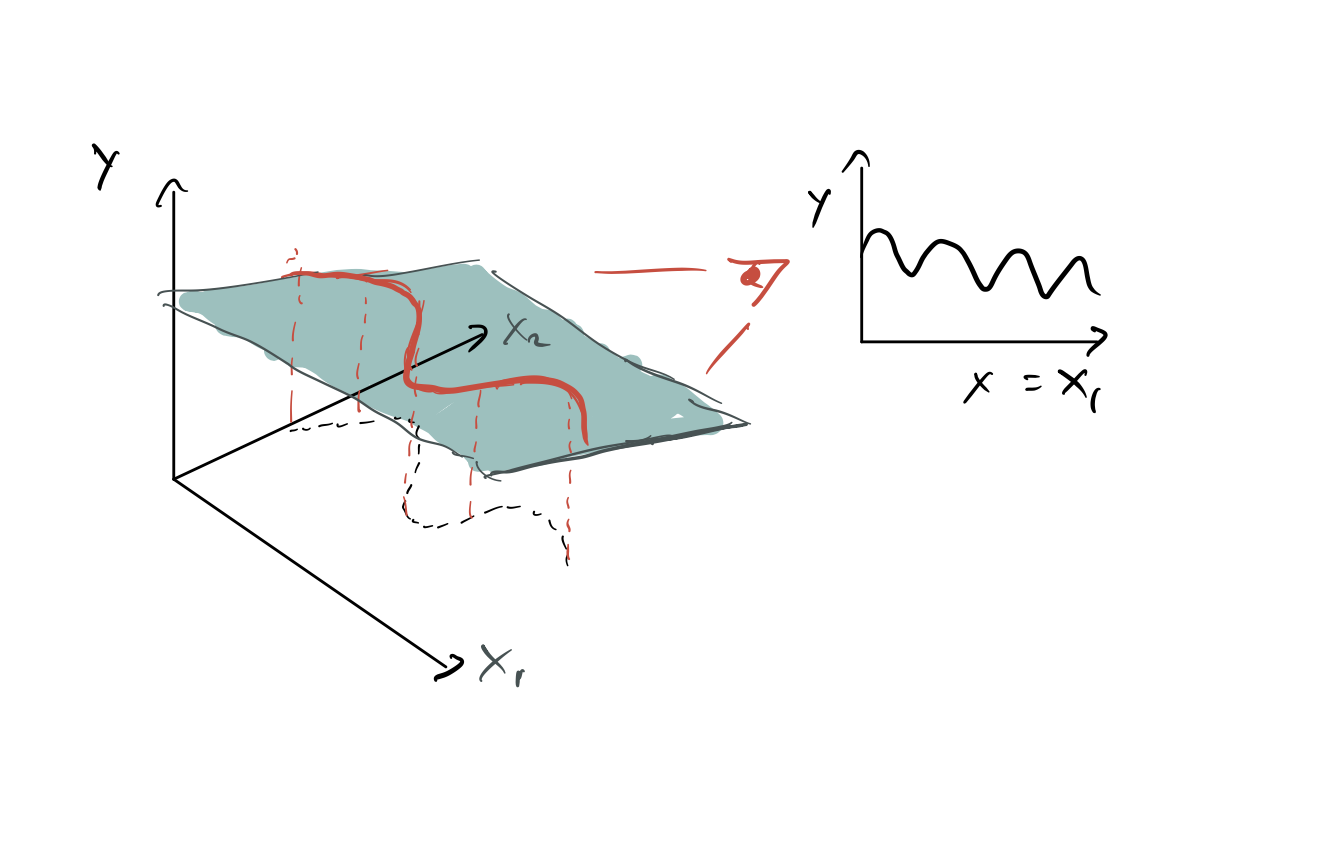
\includegraphics[width=0.8\textwidth]{feature}
    \caption{An illustration of how a nonlinear dependence on our predictor can be incorporated into the linear modeling framework by adding a feature.}
    \label{fig:feature}
\end{figure}

Which functions $\phi$ should we use? The answer of course depends on the problem at hand. For example, we might know something about the physics of the data we are modeling. In some cases, we may select the $\phi$ so that the parameters $a_i$ have clear interpretations (as is the case in linear regression model). The following illustrates such an example.  

\begin{example}
\href{https://colab.research.google.com/drive/1euwp8RjQ-fNru49tcTqVWYlqp2swGO4Y#scrollTo=heNnoCg5QWut&line=1&uniqifier=1}{Mauna Kea Data}
\end{example}




%\begin{example}
%\href{https://colab.research.google.com/drive/1euwp8RjQ-fNru49tcTqVWYlqp2swGO4Y#scrollTo=heNnoCg5QWut&line=1&uniqifier=1}{Decaying exponentials}
%\end{example}




\begin{exercise}
\href{https://colab.research.google.com/drive/1euwp8RjQ-fNru49tcTqVWYlqp2swGO4Y#scrollTo=heNnoCg5QWut&line=1&uniqifier=1}{Killing a tumor}
\end{exercise}





%\begin{example}
%\href{https://colab.research.google.com/drive/1euwp8RjQ-fNru49tcTqVWYlqp2swGO4Y#scrollTo=heNnoCg5QWut&line=1&uniqifier=1}{Complex models}
%\end{example}

\subsection{Orthogonality}
It is often to our advantage to select basis function $\phi$ which contain very different ``information".  We know from before that ideally our predictor variables should be uncorrelated, otherwise $\hat{a}_i$ will be very correlated in the sample distribution. Thus, ideally, we should select $\phi_i$ so that the correlation coefficient between $\phi_i(X)$ and $\phi_j(X)$ is very small. When 
\begin{equation}
\E[\phi_i(X)\phi_j(X)] = \E[\phi_i(X)]\E[\phi_j(X)]
\end{equation}
we say that $\phi_i$ and $\phi_j$ are {\dfn orthogonal} with respect to the distribution of $X$. We won't get too deep into this, but it's important to understand when you go looking for basis functions. One can show for example, that the basis function $\phi_{i}(x) = \sin(2\pi x)$ are orthogonal with respect to 
\begin{equation}
X \sim {\rm Uniform}(-1,1).
\end{equation}
I won't say much more on this. 

\section{Overfitting}

\subsection{Direct assessment of model predictions}

We have seen that any model has deficiencies and that {\bf expanding our model always increases $R^2$}. A natural question is: Why not make our model as complex as possible? That is, why not add as many variables as we can and nonlinear terms? A simple answer could be given with the example of a linear regression: We can't draw a line through only two points. Similarly, we can't find a unique plane in $d$ dimensions that goes through $<d$ points. This suggests we must not have more parameters in our model than data. Moreover, as the number of parameters in our model approach the amount of data, we become unable to resolve the parameters (the sample distributions become too wide) and interpret them in a meaningful way. 

However, if our goal is make predictions with a model, there is much more to the story. Even before we have nearly as many parameters as data points, our model looses its power. This is not something we can see based on the behavior of error between the model and the data, such as $R^2$, which always decreases as we expand our model. Instead, we need to look at a {\bf direct assessment of out-of-sample predictive power}. Ideally, we could look at the error between the model and the predictors for new $X$ values. One way to access this is to break our data up into two subsets, a {\dfn training}  (denoted $Y_{{\rm train},i}$) and {\dfn test} set  (denoted $Y_{{\rm test},i}$) . We fit the model using only the training set, and then see how well our model can predict the values in the test set. The following examples reveals what we can learn from this: 

\begin{example}
\href{https://colab.research.google.com/drive/1euwp8RjQ-fNru49tcTqVWYlqp2swGO4Y#scrollTo=Rz-6Ut-rrF5J}{Fitting polynomial data}
\end{example}




\subsection{Bais-variance tradeoff}
To make sense of the results in the previous example, let's define a few things. We define the training error as
\begin{equation}
\epsilon_{\rm train}^2= \E[(\hat{Y}_i - Y_{{\rm train},i})^2]
\end{equation}
where the average is taken over different realizations of our data and $\hat{Y}_i$ is our prediction of $\E[Y|X]$. Not the relationship between $R^2$ and the training error: 
\begin{equation}
R^2 \approx 1 - \frac{\epsilon_{\rm train}^2}{{\rm var}(Y_{{\rm train},i})}.
\end{equation}
Similarly, we define the test error as 
\begin{equation}
\epsilon_{\rm test}^2= \E[(\hat{Y}_i - Y_{{\rm test},i})^2]
\end{equation}
It can be shown that 
\begin{equation}
\epsilon_{\rm test}^2 = \underbrace{(\E[\hat{Y}_i]-y)^2}_{={\rm bias}}+ \underbrace{{\rm var}(\hat{Y})}_{={\rm variance}} + \sigma_{\epsilon}^2
\end{equation}

The {\dfn bias} results from the fact that our model will systematically under or over estimate the $y$ values. For example, if we try to fit an exponentially decaying curve with a straight line, different data sets will give consistent result, but on average they will overestimate the middle of the data and underestimate the ends. 

The {\dfn variance} variation between our model predictions and the data between different datasets from the same model. For example, if we interpolate every single-point, then a different set of points will cause our curve to change in ways that differ from the data. 

Roughly speaking, a biased model will give us consistent but incorrect results, while a low bias high variance model will be correct on average, but our predictions will vary a lot from data set to data set and therefore will not be reliable. {\bf Variance arrises from a model being too complex, while bias arrises from a model not being complex enough. }

\begin{figure}[h]
    \centering
    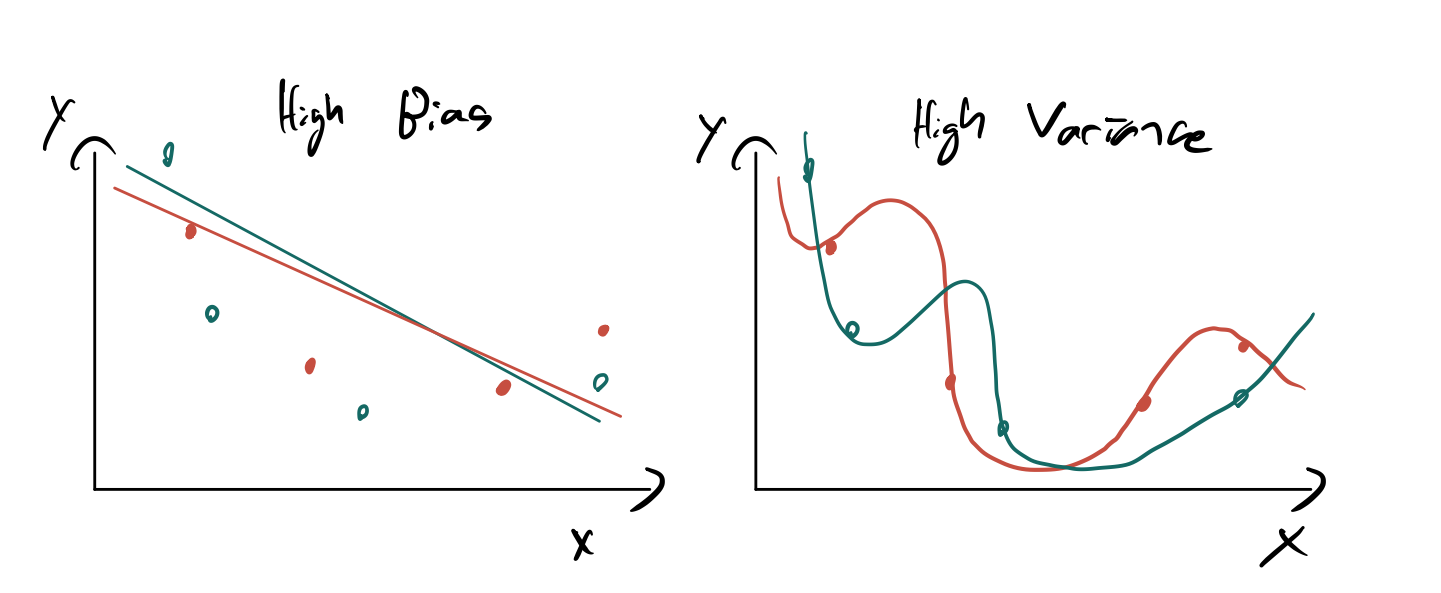
\includegraphics[width=0.8\textwidth]{bias_var}
    \caption{Bias and variance illustrated with fits to two different datasets (blue and red) drawn the from the same distribution}
    \label{fig:bv}
\end{figure}

\begin{example}
\href{https://colab.research.google.com/drive/1euwp8RjQ-fNru49tcTqVWYlqp2swGO4Y#scrollTo=q0n6Iel0auii&line=4&uniqifier=1}{Visualizing bias and variance}
\end{example}

\begin{example}
\href{https://colab.research.google.com/drive/1euwp8RjQ-fNru49tcTqVWYlqp2swGO4Y#scrollTo=myEKGetym6MD&line=1&uniqifier=1}{Which do we prefer?}
\end{example}



\subsection{Information criteria vs. cross validation}
It seems like it would be nice to access whether our model is overfitting without splitting the data up, so that (1) we are using all our data and (2) we don't need to refit the model on all the data after cross validation to get our final results. It's also a bit unsatisfying that $R^2$, which was supposed to measure a models predictive power fails to do that job so miserably as the number of parameters grows. This had motivated a number of alternative metrics for selecting the ``best" model which do not relay on out of sample tests. One example is the Akaike information criterion (AIC), which is defined as 
\begin{equation}
{\rm AIC} = 2k - 2\ln \sum (\hat{Y}_i - Y_i)^2.
\end{equation}
We prefer models where AIC is small, so the AIC rewards models where $\hat{Y}_i$ and close to $Y_i$, but penalizes the number of parameters. This seems reasonable, but it's not clear that this is the correct way to penalize parameters. For example, why is AIC linear in $k$? Why does the $k$ term not depend on how much data we have? There are other information criteria one could use, but they have similar issues. I prefer to simply use cross validation. 

The following example illustrates how the AIC doesn't tell us if we are overfitting. 
\begin{example}
\href{https://colab.research.google.com/drive/1euwp8RjQ-fNru49tcTqVWYlqp2swGO4Y#scrollTo=myEKGetym6MD&line=1&uniqifier=1}{AIC}
\end{example}

\section{Additional examples}

\begin{example}
\href{https://colab.research.google.com/drive/1euwp8RjQ-fNru49tcTqVWYlqp2swGO4Y#scrollTo=Rz-6Ut-rrF5J}{Earnings data}
\end{example}




%
%\begin{example}
%\href{}{Thinking about the project}
%\end{example} 
%%\begin{example}
%%\href{s}{Fitting polynomial data}
%%\end{example}
%\begin{exercise}
%\href{}{Thinking about the project}
%\end{exercise}


